\documentclass[twoside]{book}

% Packages required by doxygen
\usepackage{fixltx2e}
\usepackage{calc}
\usepackage{doxygen}
\usepackage{graphicx}
\usepackage[utf8]{inputenc}
\usepackage{makeidx}
\usepackage{multicol}
\usepackage{multirow}
\PassOptionsToPackage{warn}{textcomp}
\usepackage{textcomp}
\usepackage[nointegrals]{wasysym}
\usepackage[table]{xcolor}

% Font selection
\usepackage[T1]{fontenc}
\usepackage{mathptmx}
\usepackage[scaled=.90]{helvet}
\usepackage{courier}
\usepackage{amssymb}
\usepackage{sectsty}
\renewcommand{\familydefault}{\sfdefault}
\allsectionsfont{%
  \fontseries{bc}\selectfont%
  \color{darkgray}%
}
\renewcommand{\DoxyLabelFont}{%
  \fontseries{bc}\selectfont%
  \color{darkgray}%
}
\newcommand{\+}{\discretionary{\mbox{\scriptsize$\hookleftarrow$}}{}{}}

% Page & text layout
\usepackage{geometry}
\geometry{%
  a4paper,%
  top=2.5cm,%
  bottom=2.5cm,%
  left=2.5cm,%
  right=2.5cm%
}
\tolerance=750
\hfuzz=15pt
\hbadness=750
\setlength{\emergencystretch}{15pt}
\setlength{\parindent}{0cm}
\setlength{\parskip}{0.2cm}
\makeatletter
\renewcommand{\paragraph}{%
  \@startsection{paragraph}{4}{0ex}{-1.0ex}{1.0ex}{%
    \normalfont\normalsize\bfseries\SS@parafont%
  }%
}
\renewcommand{\subparagraph}{%
  \@startsection{subparagraph}{5}{0ex}{-1.0ex}{1.0ex}{%
    \normalfont\normalsize\bfseries\SS@subparafont%
  }%
}
\makeatother

% Headers & footers
\usepackage{fancyhdr}
\pagestyle{fancyplain}
\fancyhead[LE]{\fancyplain{}{\bfseries\thepage}}
\fancyhead[CE]{\fancyplain{}{}}
\fancyhead[RE]{\fancyplain{}{\bfseries\leftmark}}
\fancyhead[LO]{\fancyplain{}{\bfseries\rightmark}}
\fancyhead[CO]{\fancyplain{}{}}
\fancyhead[RO]{\fancyplain{}{\bfseries\thepage}}
\fancyfoot[LE]{\fancyplain{}{}}
\fancyfoot[CE]{\fancyplain{}{}}
\fancyfoot[RE]{\fancyplain{}{\bfseries\scriptsize Generated on Wed May 6 2015 23\+:57\+:39 for Kraj(2) by Doxygen }}
\fancyfoot[LO]{\fancyplain{}{\bfseries\scriptsize Generated on Wed May 6 2015 23\+:57\+:39 for Kraj(2) by Doxygen }}
\fancyfoot[CO]{\fancyplain{}{}}
\fancyfoot[RO]{\fancyplain{}{}}
\renewcommand{\footrulewidth}{0.4pt}
\renewcommand{\chaptermark}[1]{%
  \markboth{#1}{}%
}
\renewcommand{\sectionmark}[1]{%
  \markright{\thesection\ #1}%
}

% Indices & bibliography
\usepackage{natbib}
\usepackage[titles]{tocloft}
\setcounter{tocdepth}{3}
\setcounter{secnumdepth}{5}
\makeindex

% Custom commands
\newcommand{\clearemptydoublepage}{%
  \newpage{\pagestyle{empty}\cleardoublepage}%
}


%===== C O N T E N T S =====

\begin{document}

% Titlepage & ToC
\pagenumbering{roman}
\begin{titlepage}
\vspace*{7cm}
\begin{center}%
{\Large Kraj(2) }\\
\vspace*{1cm}
{\large Generated by Doxygen 1.8.8}\\
\vspace*{0.5cm}
{\small Wed May 6 2015 23:57:39}\\
\end{center}
\end{titlepage}
\clearemptydoublepage
\tableofcontents
\clearemptydoublepage
\pagenumbering{arabic}

%--- Begin generated contents ---
\chapter{Kraj\+:\+: Strona g��wna}
\label{index}Programowanie obiektowe -\/ Projekt nr 2~\newline
Implementowany obiekt\+: \doxyref{Kraj}{p.}{class_kraj}~\newline
~\newline

\chapter{Hierarchical Index}
\section{Class Hierarchy}
This inheritance list is sorted roughly, but not completely, alphabetically\+:\begin{DoxyCompactList}
\item \contentsline{section}{Czesc\+\_\+\+Swiata}{\pageref{class_czesc___swiata}}{}
\begin{DoxyCompactList}
\item \contentsline{section}{Kraj}{\pageref{class_kraj}}{}
\begin{DoxyCompactList}
\item \contentsline{section}{Demokratyczny}{\pageref{class_demokratyczny}}{}
\item \contentsline{section}{Socjalistyczny}{\pageref{class_socjalistyczny}}{}
\end{DoxyCompactList}
\end{DoxyCompactList}
\item \contentsline{section}{Polityka}{\pageref{class_polityka}}{}
\item \contentsline{section}{Terytorium}{\pageref{class_terytorium}}{}
\end{DoxyCompactList}

\chapter{Class Index}
\section{Class List}
Here are the classes, structs, unions and interfaces with brief descriptions\+:\begin{DoxyCompactList}
\item\contentsline{section}{{\bf Czesc\+\_\+\+Swiata} \\*Klasa abstrakcyjna }{\pageref{class_czesc___swiata}}{}
\item\contentsline{section}{{\bf Demokratyczny} \\*Klasa \doxyref{Demokratyczny}{p.}{class_demokratyczny}, pochodna klasy \doxyref{Kraj}{p.}{class_kraj} }{\pageref{class_demokratyczny}}{}
\item\contentsline{section}{{\bf Kraj} \\*Klasa \doxyref{Kraj}{p.}{class_kraj}, pochodna klasy \doxyref{Czesc\+\_\+\+Swiata}{p.}{class_czesc___swiata} }{\pageref{class_kraj}}{}
\item\contentsline{section}{{\bf Polityka} \\*Klasa \doxyref{Polityka}{p.}{class_polityka}, podklasa klasy \doxyref{Kraj}{p.}{class_kraj} }{\pageref{class_polityka}}{}
\item\contentsline{section}{{\bf Socjalistyczny} \\*Klasa \doxyref{Socjalistyczny}{p.}{class_socjalistyczny}, pochodna klasy \doxyref{Kraj}{p.}{class_kraj} }{\pageref{class_socjalistyczny}}{}
\item\contentsline{section}{{\bf Terytorium} \\*Klasa \doxyref{Terytorium}{p.}{class_terytorium}, podklasa klasy \doxyref{Kraj}{p.}{class_kraj} }{\pageref{class_terytorium}}{}
\end{DoxyCompactList}

\chapter{File Index}
\section{File List}
Here is a list of all files with brief descriptions\+:\begin{DoxyCompactList}
\item\contentsline{section}{{\bf Czesc\+\_\+\+Swiata.\+cpp} }{\pageref{_czesc___swiata_8cpp}}{}
\item\contentsline{section}{{\bf Czesc\+\_\+\+Swiata.\+h} }{\pageref{_czesc___swiata_8h}}{}
\item\contentsline{section}{{\bf Demokratyczny.\+cpp} }{\pageref{_demokratyczny_8cpp}}{}
\item\contentsline{section}{{\bf Demokratyczny.\+h} }{\pageref{_demokratyczny_8h}}{}
\item\contentsline{section}{{\bf Kraj-\/2.\+cpp} }{\pageref{_kraj-2_8cpp}}{}
\item\contentsline{section}{{\bf Kraj.\+cpp} }{\pageref{_kraj_8cpp}}{}
\item\contentsline{section}{{\bf Kraj.\+h} }{\pageref{_kraj_8h}}{}
\item\contentsline{section}{{\bf Polityka.\+cpp} }{\pageref{_polityka_8cpp}}{}
\item\contentsline{section}{{\bf Polityka.\+h} }{\pageref{_polityka_8h}}{}
\item\contentsline{section}{{\bf Socjalistyczny.\+cpp} }{\pageref{_socjalistyczny_8cpp}}{}
\item\contentsline{section}{{\bf Socjalistyczny.\+h} }{\pageref{_socjalistyczny_8h}}{}
\item\contentsline{section}{{\bf stdafx.\+cpp} }{\pageref{stdafx_8cpp}}{}
\item\contentsline{section}{{\bf stdafx.\+h} }{\pageref{stdafx_8h}}{}
\item\contentsline{section}{{\bf targetver.\+h} }{\pageref{targetver_8h}}{}
\item\contentsline{section}{{\bf Terytorium.\+cpp} }{\pageref{_terytorium_8cpp}}{}
\item\contentsline{section}{{\bf Terytorium.\+h} }{\pageref{_terytorium_8h}}{}
\end{DoxyCompactList}

\chapter{Class Documentation}
\section{Czesc\+\_\+\+Swiata Class Reference}
\label{class_czesc___swiata}\index{Czesc\+\_\+\+Swiata@{Czesc\+\_\+\+Swiata}}


Klasa abstrakcyjna.  




{\ttfamily \#include $<$Czesc\+\_\+\+Swiata.\+h$>$}

Inheritance diagram for Czesc\+\_\+\+Swiata\+:\begin{figure}[H]
\begin{center}
\leavevmode
\includegraphics[height=3.000000cm]{class_czesc___swiata}
\end{center}
\end{figure}
\subsection*{Public Member Functions}
\begin{DoxyCompactItemize}
\item 
{\bf Czesc\+\_\+\+Swiata} ()
\begin{DoxyCompactList}\small\item\em Kontruktor domy�lny. \end{DoxyCompactList}\item 
virtual {\bf $\sim$\+Czesc\+\_\+\+Swiata} ()
\begin{DoxyCompactList}\small\item\em Destruktor wirtualny. \end{DoxyCompactList}\item 
virtual void {\bf zmien\+Zmienna} (int nowa\+\_\+wartosc)=0
\begin{DoxyCompactList}\small\item\em Procedura wirtualna. \end{DoxyCompactList}\item 
virtual void {\bf pokaz\+Stan} ()=0
\begin{DoxyCompactList}\small\item\em Procedura wirtualna. \end{DoxyCompactList}\end{DoxyCompactItemize}
\subsection*{Friends}
\begin{DoxyCompactItemize}
\item 
std\+::ostream \& {\bf operator$<$$<$} (std\+::ostream \&s, {\bf Czesc\+\_\+\+Swiata} \&czesc)
\begin{DoxyCompactList}\small\item\em Operator strumieniowy $<$$<$. \end{DoxyCompactList}\item 
std\+::istream \& {\bf operator$>$$>$} (std\+::istream \&s, {\bf Czesc\+\_\+\+Swiata} \&czesc)
\begin{DoxyCompactList}\small\item\em Operator strumieniowy $>$$>$ \end{DoxyCompactList}\end{DoxyCompactItemize}


\subsection{Detailed Description}
Klasa abstrakcyjna. 

\subsection{Constructor \& Destructor Documentation}
\index{Czesc\+\_\+\+Swiata@{Czesc\+\_\+\+Swiata}!Czesc\+\_\+\+Swiata@{Czesc\+\_\+\+Swiata}}
\index{Czesc\+\_\+\+Swiata@{Czesc\+\_\+\+Swiata}!Czesc\+\_\+\+Swiata@{Czesc\+\_\+\+Swiata}}
\subsubsection[{Czesc\+\_\+\+Swiata}]{\setlength{\rightskip}{0pt plus 5cm}Czesc\+\_\+\+Swiata\+::\+Czesc\+\_\+\+Swiata (
\begin{DoxyParamCaption}
{}
\end{DoxyParamCaption}
)}\label{class_czesc___swiata_aab68757ac91477745bea68195bcba020}


Kontruktor domy�lny. 

\index{Czesc\+\_\+\+Swiata@{Czesc\+\_\+\+Swiata}!````~Czesc\+\_\+\+Swiata@{$\sim$\+Czesc\+\_\+\+Swiata}}
\index{````~Czesc\+\_\+\+Swiata@{$\sim$\+Czesc\+\_\+\+Swiata}!Czesc\+\_\+\+Swiata@{Czesc\+\_\+\+Swiata}}
\subsubsection[{$\sim$\+Czesc\+\_\+\+Swiata}]{\setlength{\rightskip}{0pt plus 5cm}Czesc\+\_\+\+Swiata\+::$\sim$\+Czesc\+\_\+\+Swiata (
\begin{DoxyParamCaption}
{}
\end{DoxyParamCaption}
)\hspace{0.3cm}{\ttfamily [virtual]}}\label{class_czesc___swiata_a429678b1f60fc8f3a23b7e92ba8aa819}


Destruktor wirtualny. 



\subsection{Member Function Documentation}
\index{Czesc\+\_\+\+Swiata@{Czesc\+\_\+\+Swiata}!pokaz\+Stan@{pokaz\+Stan}}
\index{pokaz\+Stan@{pokaz\+Stan}!Czesc\+\_\+\+Swiata@{Czesc\+\_\+\+Swiata}}
\subsubsection[{pokaz\+Stan}]{\setlength{\rightskip}{0pt plus 5cm}virtual void Czesc\+\_\+\+Swiata\+::pokaz\+Stan (
\begin{DoxyParamCaption}
{}
\end{DoxyParamCaption}
)\hspace{0.3cm}{\ttfamily [pure virtual]}}\label{class_czesc___swiata_a9b4d99ec5e00665b61da321c76deedb7}


Procedura wirtualna. 



Implemented in {\bf Kraj} \doxyref{}{p.}{class_kraj_a295b213055a7a781102eab5be6bad838}.

\index{Czesc\+\_\+\+Swiata@{Czesc\+\_\+\+Swiata}!zmien\+Zmienna@{zmien\+Zmienna}}
\index{zmien\+Zmienna@{zmien\+Zmienna}!Czesc\+\_\+\+Swiata@{Czesc\+\_\+\+Swiata}}
\subsubsection[{zmien\+Zmienna}]{\setlength{\rightskip}{0pt plus 5cm}virtual void Czesc\+\_\+\+Swiata\+::zmien\+Zmienna (
\begin{DoxyParamCaption}
\item[{int}]{nowa\+\_\+wartosc}
\end{DoxyParamCaption}
)\hspace{0.3cm}{\ttfamily [pure virtual]}}\label{class_czesc___swiata_a8295ea01dffb9e0c677d7f167ac5bc1c}


Procedura wirtualna. 



Implemented in {\bf Kraj} \doxyref{}{p.}{class_kraj_a07fbb8117dfc5910069a9dbabbc50d03}, {\bf Demokratyczny} \doxyref{}{p.}{class_demokratyczny_aeb2e9bad6d5f6604c6ea2cc82c1372d1}, and {\bf Socjalistyczny} \doxyref{}{p.}{class_socjalistyczny_a69f80e5d7d825d99d53a0c5340bc2801}.



\subsection{Friends And Related Function Documentation}
\index{Czesc\+\_\+\+Swiata@{Czesc\+\_\+\+Swiata}!operator$<$$<$@{operator$<$$<$}}
\index{operator$<$$<$@{operator$<$$<$}!Czesc\+\_\+\+Swiata@{Czesc\+\_\+\+Swiata}}
\subsubsection[{operator$<$$<$}]{\setlength{\rightskip}{0pt plus 5cm}std\+::ostream\& operator$<$$<$ (
\begin{DoxyParamCaption}
\item[{std\+::ostream \&}]{s, }
\item[{{\bf Czesc\+\_\+\+Swiata} \&}]{czesc}
\end{DoxyParamCaption}
)\hspace{0.3cm}{\ttfamily [friend]}}\label{class_czesc___swiata_a1d68849ebe88bd9ceb7567df9c0c0bc5}


Operator strumieniowy $<$$<$. 

\index{Czesc\+\_\+\+Swiata@{Czesc\+\_\+\+Swiata}!operator$>$$>$@{operator$>$$>$}}
\index{operator$>$$>$@{operator$>$$>$}!Czesc\+\_\+\+Swiata@{Czesc\+\_\+\+Swiata}}
\subsubsection[{operator$>$$>$}]{\setlength{\rightskip}{0pt plus 5cm}std\+::istream\& operator$>$$>$ (
\begin{DoxyParamCaption}
\item[{std\+::istream \&}]{s, }
\item[{{\bf Czesc\+\_\+\+Swiata} \&}]{czesc}
\end{DoxyParamCaption}
)\hspace{0.3cm}{\ttfamily [friend]}}\label{class_czesc___swiata_af23046cfaf8a4601645c7e8429eb8b54}


Operator strumieniowy $>$$>$ 



The documentation for this class was generated from the following files\+:\begin{DoxyCompactItemize}
\item 
{\bf Czesc\+\_\+\+Swiata.\+h}\item 
{\bf Czesc\+\_\+\+Swiata.\+cpp}\end{DoxyCompactItemize}

\section{Demokratyczny Class Reference}
\label{class_demokratyczny}\index{Demokratyczny@{Demokratyczny}}


Klasa \doxyref{Demokratyczny}{p.}{class_demokratyczny}, pochodna klasy \doxyref{Kraj}{p.}{class_kraj}.  




{\ttfamily \#include $<$Demokratyczny.\+h$>$}

Inheritance diagram for Demokratyczny\+:\begin{figure}[H]
\begin{center}
\leavevmode
\includegraphics[height=3.000000cm]{class_demokratyczny}
\end{center}
\end{figure}
\subsection*{Public Member Functions}
\begin{DoxyCompactItemize}
\item 
{\bf Demokratyczny} ()
\begin{DoxyCompactList}\small\item\em Kontruktor domy�lny. \end{DoxyCompactList}\item 
{\bf $\sim$\+Demokratyczny} ()
\begin{DoxyCompactList}\small\item\em Destruktor. \end{DoxyCompactList}\item 
void {\bf zmien\+Zmienna} (int nowa\+\_\+wartosc)
\begin{DoxyCompactList}\small\item\em Procedura wirtualna zmienia parametr obiektu. \end{DoxyCompactList}\item 
void {\bf zapisz\+Stan} ({\bf Demokratyczny} \&kraj)
\begin{DoxyCompactList}\small\item\em Procedura zapisuj�ca aktualny stan obiektu do pliku. \end{DoxyCompactList}\item 
void {\bf wczytaj\+Stan} ({\bf Demokratyczny} \&kraj)
\begin{DoxyCompactList}\small\item\em Procedura wczytuj�ca aktualny stan obiektu z pliku. \end{DoxyCompactList}\item 
void {\bf wyswietl\+Stan} ()
\begin{DoxyCompactList}\small\item\em Procedura wirtualna wy�wietlaj�ca aktualny stan obietku. \end{DoxyCompactList}\end{DoxyCompactItemize}
\subsection*{Friends}
\begin{DoxyCompactItemize}
\item 
std\+::ostream \& {\bf operator$<$$<$} (std\+::ostream \&s, {\bf Demokratyczny} \&demokratyczny)
\begin{DoxyCompactList}\small\item\em Operator strumieniowy $<$$<$. \end{DoxyCompactList}\item 
std\+::istream \& {\bf operator$>$$>$} (std\+::istream \&s, {\bf Demokratyczny} \&demokratyczny)
\begin{DoxyCompactList}\small\item\em Operator strumieniowy $>$$>$ \end{DoxyCompactList}\end{DoxyCompactItemize}
\subsection*{Additional Inherited Members}


\subsection{Detailed Description}
Klasa \doxyref{Demokratyczny}{p.}{class_demokratyczny}, pochodna klasy \doxyref{Kraj}{p.}{class_kraj}. 

\subsection{Constructor \& Destructor Documentation}
\index{Demokratyczny@{Demokratyczny}!Demokratyczny@{Demokratyczny}}
\index{Demokratyczny@{Demokratyczny}!Demokratyczny@{Demokratyczny}}
\subsubsection[{Demokratyczny}]{\setlength{\rightskip}{0pt plus 5cm}Demokratyczny\+::\+Demokratyczny (
\begin{DoxyParamCaption}
{}
\end{DoxyParamCaption}
)}\label{class_demokratyczny_ad06e7a17eee6342b4c3ef5538836b06a}


Kontruktor domy�lny. 

\index{Demokratyczny@{Demokratyczny}!````~Demokratyczny@{$\sim$\+Demokratyczny}}
\index{````~Demokratyczny@{$\sim$\+Demokratyczny}!Demokratyczny@{Demokratyczny}}
\subsubsection[{$\sim$\+Demokratyczny}]{\setlength{\rightskip}{0pt plus 5cm}Demokratyczny\+::$\sim$\+Demokratyczny (
\begin{DoxyParamCaption}
{}
\end{DoxyParamCaption}
)}\label{class_demokratyczny_ac8ac8bb839b7d4b6c7fb323aead914a6}


Destruktor. 



\subsection{Member Function Documentation}
\index{Demokratyczny@{Demokratyczny}!wczytaj\+Stan@{wczytaj\+Stan}}
\index{wczytaj\+Stan@{wczytaj\+Stan}!Demokratyczny@{Demokratyczny}}
\subsubsection[{wczytaj\+Stan}]{\setlength{\rightskip}{0pt plus 5cm}void Demokratyczny\+::wczytaj\+Stan (
\begin{DoxyParamCaption}
\item[{{\bf Demokratyczny} \&}]{kraj}
\end{DoxyParamCaption}
)}\label{class_demokratyczny_a7a466fc89602845f7a92b1e025d0fd4d}


Procedura wczytuj�ca aktualny stan obiektu z pliku. 

\index{Demokratyczny@{Demokratyczny}!wyswietl\+Stan@{wyswietl\+Stan}}
\index{wyswietl\+Stan@{wyswietl\+Stan}!Demokratyczny@{Demokratyczny}}
\subsubsection[{wyswietl\+Stan}]{\setlength{\rightskip}{0pt plus 5cm}void Demokratyczny\+::wyswietl\+Stan (
\begin{DoxyParamCaption}
{}
\end{DoxyParamCaption}
)}\label{class_demokratyczny_a43e42fc5840ab7c763a57e5092071654}


Procedura wirtualna wy�wietlaj�ca aktualny stan obietku. 

\index{Demokratyczny@{Demokratyczny}!zapisz\+Stan@{zapisz\+Stan}}
\index{zapisz\+Stan@{zapisz\+Stan}!Demokratyczny@{Demokratyczny}}
\subsubsection[{zapisz\+Stan}]{\setlength{\rightskip}{0pt plus 5cm}void Demokratyczny\+::zapisz\+Stan (
\begin{DoxyParamCaption}
\item[{{\bf Demokratyczny} \&}]{kraj}
\end{DoxyParamCaption}
)}\label{class_demokratyczny_a50899f654d7235391316c0c7f95ef472}


Procedura zapisuj�ca aktualny stan obiektu do pliku. 

\index{Demokratyczny@{Demokratyczny}!zmien\+Zmienna@{zmien\+Zmienna}}
\index{zmien\+Zmienna@{zmien\+Zmienna}!Demokratyczny@{Demokratyczny}}
\subsubsection[{zmien\+Zmienna}]{\setlength{\rightskip}{0pt plus 5cm}void Demokratyczny\+::zmien\+Zmienna (
\begin{DoxyParamCaption}
\item[{int}]{nowa\+\_\+wartosc}
\end{DoxyParamCaption}
)\hspace{0.3cm}{\ttfamily [virtual]}}\label{class_demokratyczny_aeb2e9bad6d5f6604c6ea2cc82c1372d1}


Procedura wirtualna zmienia parametr obiektu. 



Implements {\bf Czesc\+\_\+\+Swiata} \doxyref{}{p.}{class_czesc___swiata_a8295ea01dffb9e0c677d7f167ac5bc1c}.



\subsection{Friends And Related Function Documentation}
\index{Demokratyczny@{Demokratyczny}!operator$<$$<$@{operator$<$$<$}}
\index{operator$<$$<$@{operator$<$$<$}!Demokratyczny@{Demokratyczny}}
\subsubsection[{operator$<$$<$}]{\setlength{\rightskip}{0pt plus 5cm}std\+::ostream\& operator$<$$<$ (
\begin{DoxyParamCaption}
\item[{std\+::ostream \&}]{s, }
\item[{{\bf Demokratyczny} \&}]{demokratyczny}
\end{DoxyParamCaption}
)\hspace{0.3cm}{\ttfamily [friend]}}\label{class_demokratyczny_ad7864b9cd701a8e1cc4571218a40ee65}


Operator strumieniowy $<$$<$. 

\index{Demokratyczny@{Demokratyczny}!operator$>$$>$@{operator$>$$>$}}
\index{operator$>$$>$@{operator$>$$>$}!Demokratyczny@{Demokratyczny}}
\subsubsection[{operator$>$$>$}]{\setlength{\rightskip}{0pt plus 5cm}std\+::istream\& operator$>$$>$ (
\begin{DoxyParamCaption}
\item[{std\+::istream \&}]{s, }
\item[{{\bf Demokratyczny} \&}]{demokratyczny}
\end{DoxyParamCaption}
)\hspace{0.3cm}{\ttfamily [friend]}}\label{class_demokratyczny_a8054b20cbce11328d6335d171d6ee9f8}


Operator strumieniowy $>$$>$ 



The documentation for this class was generated from the following files\+:\begin{DoxyCompactItemize}
\item 
{\bf Demokratyczny.\+h}\item 
{\bf Demokratyczny.\+cpp}\end{DoxyCompactItemize}

\section{Kraj Class Reference}
\label{class_kraj}\index{Kraj@{Kraj}}


Klasa \doxyref{Kraj}{p.}{class_kraj}, pochodna klasy \doxyref{Czesc\+\_\+\+Swiata}{p.}{class_czesc___swiata}.  




{\ttfamily \#include $<$Kraj.\+h$>$}

Inheritance diagram for Kraj\+:\begin{figure}[H]
\begin{center}
\leavevmode
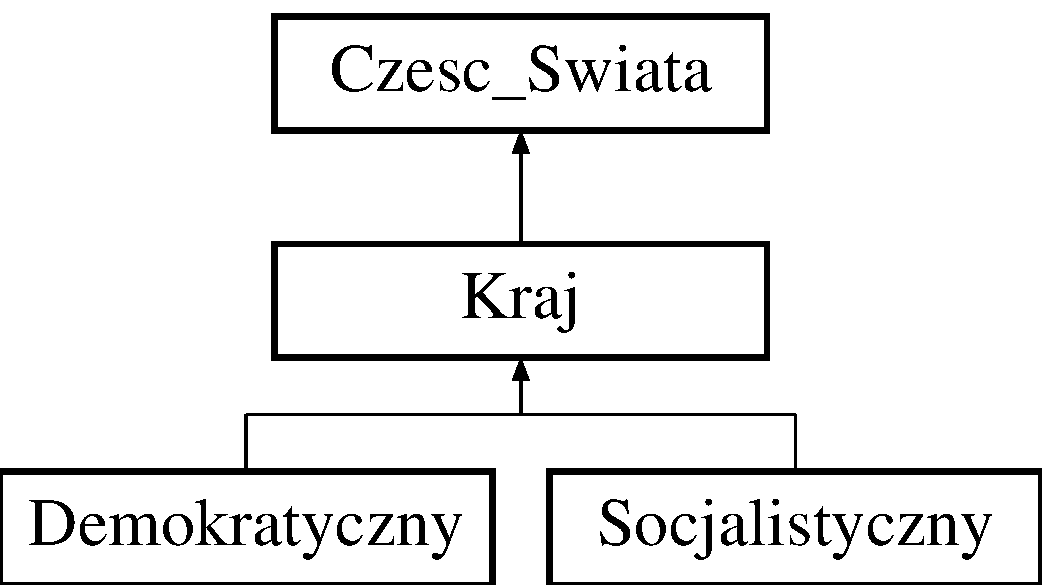
\includegraphics[height=3.000000cm]{class_kraj}
\end{center}
\end{figure}
\subsection*{Public Member Functions}
\begin{DoxyCompactItemize}
\item 
{\bf Kraj} ()
\begin{DoxyCompactList}\small\item\em Kontruktor domy�lny. \end{DoxyCompactList}\item 
{\bf Kraj} (int liczba\+\_\+s)
\begin{DoxyCompactList}\small\item\em Kontruktor. \end{DoxyCompactList}\item 
{\bf $\sim$\+Kraj} ()
\begin{DoxyCompactList}\small\item\em Destruktor. \end{DoxyCompactList}\item 
{\bf Kraj} (const {\bf Kraj} \&kraj)
\begin{DoxyCompactList}\small\item\em Konstruktor kopiujacy. \end{DoxyCompactList}\item 
void {\bf zmien\+Imie\+Zalozyciela} (string {\bf nowe\+\_\+imie})
\begin{DoxyCompactList}\small\item\em Procedura modyfikuj�ca pole imie zalozyciela. \end{DoxyCompactList}\item 
void {\bf zmien\+Nazwe} (string {\bf nowa\+\_\+nazwa})
\begin{DoxyCompactList}\small\item\em Procedura modyfikuj�ca pole nazwa. \end{DoxyCompactList}\item 
void {\bf zmien\+Liczbe\+Sasiadow} (string nowa\+\_\+liczba\+\_\+sasiadow)
\begin{DoxyCompactList}\small\item\em Procedura modyfikuj�ca pole ocena. \end{DoxyCompactList}\item 
void {\bf pokaz\+Stan} ()
\begin{DoxyCompactList}\small\item\em Procedura wirtualna wy�wietlaj�ca aktualny stan obietku. \end{DoxyCompactList}\item 
void {\bf wyswietl\+Ilosc\+Obiektow} ()
\begin{DoxyCompactList}\small\item\em Procedura wyswielaj�ca ilo�� stworzonych obiekt�w \end{DoxyCompactList}\item 
void {\bf wyswietl\+Nazwe} ()
\begin{DoxyCompactList}\small\item\em Procedura wy�wietlaj�ca nazwe obiektu. \end{DoxyCompactList}\item 
void {\bf zapisz\+Stan} ({\bf Kraj} \&kraj)
\begin{DoxyCompactList}\small\item\em Procedura zapisuj�ca aktualny stan obiektu. \end{DoxyCompactList}\item 
void {\bf wczytaj\+Stan} ({\bf Kraj} \&kraj)
\begin{DoxyCompactList}\small\item\em Procedura wczytuj�ca aktualny stan obiektu. \end{DoxyCompactList}\item 
void {\bf zmien\+Zmienna} (int nowa\+\_\+wartosc)
\begin{DoxyCompactList}\small\item\em Procedura wirtualna zmieniaj�ca wybrana zmienna obiektu. \end{DoxyCompactList}\end{DoxyCompactItemize}
\subsection*{Static Public Attributes}
\begin{DoxyCompactItemize}
\item 
static int {\bf liczba\+\_\+obiektow} = 0
\begin{DoxyCompactList}\small\item\em Zmienna statyczna, przechowuje liczbe utworzonych obiektow. \end{DoxyCompactList}\end{DoxyCompactItemize}
\subsection*{Protected Attributes}
\begin{DoxyCompactItemize}
\item 
string {\bf nazwa}
\begin{DoxyCompactList}\small\item\em zmienna przechowuj�ca nazwe Kraju \end{DoxyCompactList}\item 
string {\bf imie\+\_\+zalozyciela}
\begin{DoxyCompactList}\small\item\em zmienna przechowuj�ca imie zalozyciela kraju \end{DoxyCompactList}\item 
int {\bf liczba\+\_\+sasiadow}
\begin{DoxyCompactList}\small\item\em zmienna przechowuj�ca liczbe sasiednich krajow \end{DoxyCompactList}\end{DoxyCompactItemize}
\subsection*{Friends}
\begin{DoxyCompactItemize}
\item 
std\+::ostream \& {\bf operator$<$$<$} (std\+::ostream \&s, {\bf Kraj} \&kraj)
\begin{DoxyCompactList}\small\item\em Operator strumieniowy $<$$<$. \end{DoxyCompactList}\item 
std\+::istream \& {\bf operator$>$$>$} (std\+::istream \&s, {\bf Kraj} \&kraj)
\begin{DoxyCompactList}\small\item\em Operator strumieniowy $>$$>$ \end{DoxyCompactList}\end{DoxyCompactItemize}


\subsection{Detailed Description}
Klasa \doxyref{Kraj}{p.}{class_kraj}, pochodna klasy \doxyref{Czesc\+\_\+\+Swiata}{p.}{class_czesc___swiata}. 

\subsection{Constructor \& Destructor Documentation}
\index{Kraj@{Kraj}!Kraj@{Kraj}}
\index{Kraj@{Kraj}!Kraj@{Kraj}}
\subsubsection[{Kraj}]{\setlength{\rightskip}{0pt plus 5cm}Kraj\+::\+Kraj (
\begin{DoxyParamCaption}
{}
\end{DoxyParamCaption}
)}\label{class_kraj_a8b8539fa574725fe1227ed75b05cb89d}


Kontruktor domy�lny. 

\index{Kraj@{Kraj}!Kraj@{Kraj}}
\index{Kraj@{Kraj}!Kraj@{Kraj}}
\subsubsection[{Kraj}]{\setlength{\rightskip}{0pt plus 5cm}Kraj\+::\+Kraj (
\begin{DoxyParamCaption}
\item[{int}]{liczba\+\_\+s}
\end{DoxyParamCaption}
)}\label{class_kraj_a8e8765d13e7e1c19afff0ed72c12846a}


Kontruktor. 

\index{Kraj@{Kraj}!````~Kraj@{$\sim$\+Kraj}}
\index{````~Kraj@{$\sim$\+Kraj}!Kraj@{Kraj}}
\subsubsection[{$\sim$\+Kraj}]{\setlength{\rightskip}{0pt plus 5cm}Kraj\+::$\sim$\+Kraj (
\begin{DoxyParamCaption}
{}
\end{DoxyParamCaption}
)}\label{class_kraj_a213be9b1083f952a403d9611ed682d3a}


Destruktor. 

\index{Kraj@{Kraj}!Kraj@{Kraj}}
\index{Kraj@{Kraj}!Kraj@{Kraj}}
\subsubsection[{Kraj}]{\setlength{\rightskip}{0pt plus 5cm}Kraj\+::\+Kraj (
\begin{DoxyParamCaption}
\item[{const {\bf Kraj} \&}]{kraj}
\end{DoxyParamCaption}
)}\label{class_kraj_abafd7dd03332271012399d035281ae36}


Konstruktor kopiujacy. 



\subsection{Member Function Documentation}
\index{Kraj@{Kraj}!pokaz\+Stan@{pokaz\+Stan}}
\index{pokaz\+Stan@{pokaz\+Stan}!Kraj@{Kraj}}
\subsubsection[{pokaz\+Stan}]{\setlength{\rightskip}{0pt plus 5cm}void Kraj\+::pokaz\+Stan (
\begin{DoxyParamCaption}
{}
\end{DoxyParamCaption}
)\hspace{0.3cm}{\ttfamily [virtual]}}\label{class_kraj_a295b213055a7a781102eab5be6bad838}


Procedura wirtualna wy�wietlaj�ca aktualny stan obietku. 



Implements {\bf Czesc\+\_\+\+Swiata} \doxyref{}{p.}{class_czesc___swiata_a9b4d99ec5e00665b61da321c76deedb7}.

\index{Kraj@{Kraj}!wczytaj\+Stan@{wczytaj\+Stan}}
\index{wczytaj\+Stan@{wczytaj\+Stan}!Kraj@{Kraj}}
\subsubsection[{wczytaj\+Stan}]{\setlength{\rightskip}{0pt plus 5cm}void Kraj\+::wczytaj\+Stan (
\begin{DoxyParamCaption}
\item[{{\bf Kraj} \&}]{kraj}
\end{DoxyParamCaption}
)}\label{class_kraj_ab479a176c14ea8b8af8ee795d428cea0}


Procedura wczytuj�ca aktualny stan obiektu. 

\index{Kraj@{Kraj}!wyswietl\+Ilosc\+Obiektow@{wyswietl\+Ilosc\+Obiektow}}
\index{wyswietl\+Ilosc\+Obiektow@{wyswietl\+Ilosc\+Obiektow}!Kraj@{Kraj}}
\subsubsection[{wyswietl\+Ilosc\+Obiektow}]{\setlength{\rightskip}{0pt plus 5cm}void Kraj\+::wyswietl\+Ilosc\+Obiektow (
\begin{DoxyParamCaption}
{}
\end{DoxyParamCaption}
)}\label{class_kraj_addb1cd05b047eeffbc3ab6048decebae}


Procedura wyswielaj�ca ilo�� stworzonych obiekt�w 

\index{Kraj@{Kraj}!wyswietl\+Nazwe@{wyswietl\+Nazwe}}
\index{wyswietl\+Nazwe@{wyswietl\+Nazwe}!Kraj@{Kraj}}
\subsubsection[{wyswietl\+Nazwe}]{\setlength{\rightskip}{0pt plus 5cm}void Kraj\+::wyswietl\+Nazwe (
\begin{DoxyParamCaption}
{}
\end{DoxyParamCaption}
)}\label{class_kraj_a98e731501bbd9489a6058e21715fcec4}


Procedura wy�wietlaj�ca nazwe obiektu. 

\index{Kraj@{Kraj}!zapisz\+Stan@{zapisz\+Stan}}
\index{zapisz\+Stan@{zapisz\+Stan}!Kraj@{Kraj}}
\subsubsection[{zapisz\+Stan}]{\setlength{\rightskip}{0pt plus 5cm}void Kraj\+::zapisz\+Stan (
\begin{DoxyParamCaption}
\item[{{\bf Kraj} \&}]{kraj}
\end{DoxyParamCaption}
)}\label{class_kraj_a37463a8cdc74d4b47ca8e31c0ef6c4f9}


Procedura zapisuj�ca aktualny stan obiektu. 

\index{Kraj@{Kraj}!zmien\+Imie\+Zalozyciela@{zmien\+Imie\+Zalozyciela}}
\index{zmien\+Imie\+Zalozyciela@{zmien\+Imie\+Zalozyciela}!Kraj@{Kraj}}
\subsubsection[{zmien\+Imie\+Zalozyciela}]{\setlength{\rightskip}{0pt plus 5cm}void Kraj\+::zmien\+Imie\+Zalozyciela (
\begin{DoxyParamCaption}
\item[{string}]{nowe\+\_\+imie}
\end{DoxyParamCaption}
)}\label{class_kraj_aaf0198b45d4556fd2aa794a4aaac56b0}


Procedura modyfikuj�ca pole imie zalozyciela. 

Jako parametr podawany jest nowy imie 
\begin{DoxyParams}{Parameters}
{\em nowe\+\_\+imie} & jest nowym imieniem \\
\hline
\end{DoxyParams}
\begin{DoxyReturn}{Returns}
Funkcja nic nie zwraca 
\end{DoxyReturn}
\index{Kraj@{Kraj}!zmien\+Liczbe\+Sasiadow@{zmien\+Liczbe\+Sasiadow}}
\index{zmien\+Liczbe\+Sasiadow@{zmien\+Liczbe\+Sasiadow}!Kraj@{Kraj}}
\subsubsection[{zmien\+Liczbe\+Sasiadow}]{\setlength{\rightskip}{0pt plus 5cm}void Kraj\+::zmien\+Liczbe\+Sasiadow (
\begin{DoxyParamCaption}
\item[{string}]{nowa\+\_\+liczba\+\_\+sasiadow}
\end{DoxyParamCaption}
)}\label{class_kraj_a2da6ce379c110857bb5be72971658379}


Procedura modyfikuj�ca pole ocena. 

Jako parametr podawany jest nowa liczba sasiadow 
\begin{DoxyParams}{Parameters}
{\em nowa\+\_\+liczba\+\_\+sasiadow} & jest nowa liczba sasiadow \\
\hline
\end{DoxyParams}
\begin{DoxyReturn}{Returns}
Funkcja nic nie zwraca 
\end{DoxyReturn}
\index{Kraj@{Kraj}!zmien\+Nazwe@{zmien\+Nazwe}}
\index{zmien\+Nazwe@{zmien\+Nazwe}!Kraj@{Kraj}}
\subsubsection[{zmien\+Nazwe}]{\setlength{\rightskip}{0pt plus 5cm}void Kraj\+::zmien\+Nazwe (
\begin{DoxyParamCaption}
\item[{string}]{nowa\+\_\+nazwa}
\end{DoxyParamCaption}
)}\label{class_kraj_acd10daf70e90e836c92312e0d08642e9}


Procedura modyfikuj�ca pole nazwa. 

Jako parametr podawany jest nowa nazwa 
\begin{DoxyParams}{Parameters}
{\em nowa\+\_\+nazwa} & jest now� nazwa \\
\hline
\end{DoxyParams}
\begin{DoxyReturn}{Returns}
Funkcja nic nie zwraca 
\end{DoxyReturn}
\index{Kraj@{Kraj}!zmien\+Zmienna@{zmien\+Zmienna}}
\index{zmien\+Zmienna@{zmien\+Zmienna}!Kraj@{Kraj}}
\subsubsection[{zmien\+Zmienna}]{\setlength{\rightskip}{0pt plus 5cm}void Kraj\+::zmien\+Zmienna (
\begin{DoxyParamCaption}
\item[{int}]{nowa\+\_\+wartosc}
\end{DoxyParamCaption}
)\hspace{0.3cm}{\ttfamily [virtual]}}\label{class_kraj_a07fbb8117dfc5910069a9dbabbc50d03}


Procedura wirtualna zmieniaj�ca wybrana zmienna obiektu. 



Implements {\bf Czesc\+\_\+\+Swiata} \doxyref{}{p.}{class_czesc___swiata_a8295ea01dffb9e0c677d7f167ac5bc1c}.



Reimplemented in {\bf Socjalistyczny} \doxyref{}{p.}{class_socjalistyczny_a69f80e5d7d825d99d53a0c5340bc2801}.



\subsection{Friends And Related Function Documentation}
\index{Kraj@{Kraj}!operator$<$$<$@{operator$<$$<$}}
\index{operator$<$$<$@{operator$<$$<$}!Kraj@{Kraj}}
\subsubsection[{operator$<$$<$}]{\setlength{\rightskip}{0pt plus 5cm}std\+::ostream\& operator$<$$<$ (
\begin{DoxyParamCaption}
\item[{std\+::ostream \&}]{s, }
\item[{{\bf Kraj} \&}]{kraj}
\end{DoxyParamCaption}
)\hspace{0.3cm}{\ttfamily [friend]}}\label{class_kraj_ab3e186ad474ff42c43e01f06f59f449e}


Operator strumieniowy $<$$<$. 

\index{Kraj@{Kraj}!operator$>$$>$@{operator$>$$>$}}
\index{operator$>$$>$@{operator$>$$>$}!Kraj@{Kraj}}
\subsubsection[{operator$>$$>$}]{\setlength{\rightskip}{0pt plus 5cm}std\+::istream\& operator$>$$>$ (
\begin{DoxyParamCaption}
\item[{std\+::istream \&}]{s, }
\item[{{\bf Kraj} \&}]{kraj}
\end{DoxyParamCaption}
)\hspace{0.3cm}{\ttfamily [friend]}}\label{class_kraj_af23ead7fadff648cbae6a6b36096d322}


Operator strumieniowy $>$$>$ 



\subsection{Member Data Documentation}
\index{Kraj@{Kraj}!imie\+\_\+zalozyciela@{imie\+\_\+zalozyciela}}
\index{imie\+\_\+zalozyciela@{imie\+\_\+zalozyciela}!Kraj@{Kraj}}
\subsubsection[{imie\+\_\+zalozyciela}]{\setlength{\rightskip}{0pt plus 5cm}string Kraj\+::imie\+\_\+zalozyciela\hspace{0.3cm}{\ttfamily [protected]}}\label{class_kraj_a8f6603acd25e166cff99b35eafc29f31}


zmienna przechowuj�ca imie zalozyciela kraju 

\index{Kraj@{Kraj}!liczba\+\_\+obiektow@{liczba\+\_\+obiektow}}
\index{liczba\+\_\+obiektow@{liczba\+\_\+obiektow}!Kraj@{Kraj}}
\subsubsection[{liczba\+\_\+obiektow}]{\setlength{\rightskip}{0pt plus 5cm}int Kraj\+::liczba\+\_\+obiektow = 0\hspace{0.3cm}{\ttfamily [static]}}\label{class_kraj_ae4466d68e2a9273b31296707956a9da7}


Zmienna statyczna, przechowuje liczbe utworzonych obiektow. 

\index{Kraj@{Kraj}!liczba\+\_\+sasiadow@{liczba\+\_\+sasiadow}}
\index{liczba\+\_\+sasiadow@{liczba\+\_\+sasiadow}!Kraj@{Kraj}}
\subsubsection[{liczba\+\_\+sasiadow}]{\setlength{\rightskip}{0pt plus 5cm}int Kraj\+::liczba\+\_\+sasiadow\hspace{0.3cm}{\ttfamily [protected]}}\label{class_kraj_aea22624004288d6aa0ec7c27cdc7931f}


zmienna przechowuj�ca liczbe sasiednich krajow 

\index{Kraj@{Kraj}!nazwa@{nazwa}}
\index{nazwa@{nazwa}!Kraj@{Kraj}}
\subsubsection[{nazwa}]{\setlength{\rightskip}{0pt plus 5cm}string Kraj\+::nazwa\hspace{0.3cm}{\ttfamily [protected]}}\label{class_kraj_a4a3aa8d0ed1fdfb74f4996020d3f6b01}


zmienna przechowuj�ca nazwe Kraju 



The documentation for this class was generated from the following files\+:\begin{DoxyCompactItemize}
\item 
{\bf Kraj.\+h}\item 
{\bf Kraj.\+cpp}\end{DoxyCompactItemize}

\section{Polityka Class Reference}
\label{class_polityka}\index{Polityka@{Polityka}}


Klasa \doxyref{Polityka}{p.}{class_polityka}, podklasa klasy \doxyref{Kraj}{p.}{class_kraj}.  




{\ttfamily \#include $<$Polityka.\+h$>$}

\subsection*{Public Member Functions}
\begin{DoxyCompactItemize}
\item 
{\bf Polityka} ()
\begin{DoxyCompactList}\small\item\em Konstruktor domy�lny. \end{DoxyCompactList}\item 
{\bf $\sim$\+Polityka} ()
\begin{DoxyCompactList}\small\item\em Destruktor. \end{DoxyCompactList}\item 
void {\bf wczytaj\+Stan} ({\bf Polityka} \&param)
\begin{DoxyCompactList}\small\item\em Procedura wczytuj�ca aktualny stan obiektu z pliku. \end{DoxyCompactList}\item 
void {\bf zapisz\+Stan} ({\bf Polityka} \&param)
\begin{DoxyCompactList}\small\item\em Procedura zapisuj�ca aktualny stan obiektu do pliku. \end{DoxyCompactList}\end{DoxyCompactItemize}
\subsection*{Friends}
\begin{DoxyCompactItemize}
\item 
std\+::ostream \& {\bf operator$<$$<$} (std\+::ostream \&s, {\bf Polityka} \&polit)
\begin{DoxyCompactList}\small\item\em Operator strumieniowy $<$$<$. \end{DoxyCompactList}\item 
std\+::istream \& {\bf operator$>$$>$} (std\+::istream \&s, {\bf Polityka} \&polit)
\begin{DoxyCompactList}\small\item\em Operator strumieniowy $>$$>$ \end{DoxyCompactList}\end{DoxyCompactItemize}


\subsection{Detailed Description}
Klasa \doxyref{Polityka}{p.}{class_polityka}, podklasa klasy \doxyref{Kraj}{p.}{class_kraj}. 

\subsection{Constructor \& Destructor Documentation}
\index{Polityka@{Polityka}!Polityka@{Polityka}}
\index{Polityka@{Polityka}!Polityka@{Polityka}}
\subsubsection[{Polityka}]{\setlength{\rightskip}{0pt plus 5cm}Polityka\+::\+Polityka (
\begin{DoxyParamCaption}
{}
\end{DoxyParamCaption}
)}\label{class_polityka_adb85bf338a044fe6ee3f4e1ffa783361}


Konstruktor domy�lny. 

\index{Polityka@{Polityka}!````~Polityka@{$\sim$\+Polityka}}
\index{````~Polityka@{$\sim$\+Polityka}!Polityka@{Polityka}}
\subsubsection[{$\sim$\+Polityka}]{\setlength{\rightskip}{0pt plus 5cm}Polityka\+::$\sim$\+Polityka (
\begin{DoxyParamCaption}
{}
\end{DoxyParamCaption}
)}\label{class_polityka_aec878365aadcced422c34c7ef41c3295}


Destruktor. 



\subsection{Member Function Documentation}
\index{Polityka@{Polityka}!wczytaj\+Stan@{wczytaj\+Stan}}
\index{wczytaj\+Stan@{wczytaj\+Stan}!Polityka@{Polityka}}
\subsubsection[{wczytaj\+Stan}]{\setlength{\rightskip}{0pt plus 5cm}void Polityka\+::wczytaj\+Stan (
\begin{DoxyParamCaption}
\item[{{\bf Polityka} \&}]{param}
\end{DoxyParamCaption}
)}\label{class_polityka_ae5865f96baaa38a07e23af8d45b07ebf}


Procedura wczytuj�ca aktualny stan obiektu z pliku. 

\index{Polityka@{Polityka}!zapisz\+Stan@{zapisz\+Stan}}
\index{zapisz\+Stan@{zapisz\+Stan}!Polityka@{Polityka}}
\subsubsection[{zapisz\+Stan}]{\setlength{\rightskip}{0pt plus 5cm}void Polityka\+::zapisz\+Stan (
\begin{DoxyParamCaption}
\item[{{\bf Polityka} \&}]{param}
\end{DoxyParamCaption}
)}\label{class_polityka_a648a53783043ecf95f2d3a921757092b}


Procedura zapisuj�ca aktualny stan obiektu do pliku. 



\subsection{Friends And Related Function Documentation}
\index{Polityka@{Polityka}!operator$<$$<$@{operator$<$$<$}}
\index{operator$<$$<$@{operator$<$$<$}!Polityka@{Polityka}}
\subsubsection[{operator$<$$<$}]{\setlength{\rightskip}{0pt plus 5cm}std\+::ostream\& operator$<$$<$ (
\begin{DoxyParamCaption}
\item[{std\+::ostream \&}]{s, }
\item[{{\bf Polityka} \&}]{polit}
\end{DoxyParamCaption}
)\hspace{0.3cm}{\ttfamily [friend]}}\label{class_polityka_ad5ba104a8261bab40fc031b41e3783b9}


Operator strumieniowy $<$$<$. 

\index{Polityka@{Polityka}!operator$>$$>$@{operator$>$$>$}}
\index{operator$>$$>$@{operator$>$$>$}!Polityka@{Polityka}}
\subsubsection[{operator$>$$>$}]{\setlength{\rightskip}{0pt plus 5cm}std\+::istream\& operator$>$$>$ (
\begin{DoxyParamCaption}
\item[{std\+::istream \&}]{s, }
\item[{{\bf Polityka} \&}]{polit}
\end{DoxyParamCaption}
)\hspace{0.3cm}{\ttfamily [friend]}}\label{class_polityka_a7f0c2d842c512975157fec0b35997750}


Operator strumieniowy $>$$>$ 



The documentation for this class was generated from the following files\+:\begin{DoxyCompactItemize}
\item 
{\bf Polityka.\+h}\item 
{\bf Polityka.\+cpp}\end{DoxyCompactItemize}

\section{Socjalistyczny Class Reference}
\label{class_socjalistyczny}\index{Socjalistyczny@{Socjalistyczny}}


Klasa \doxyref{Socjalistyczny}{p.}{class_socjalistyczny}, pochodna klasy \doxyref{Kraj}{p.}{class_kraj}.  




{\ttfamily \#include $<$Socjalistyczny.\+h$>$}

Inheritance diagram for Socjalistyczny\+:\begin{figure}[H]
\begin{center}
\leavevmode
\includegraphics[height=3.000000cm]{class_socjalistyczny}
\end{center}
\end{figure}
\subsection*{Public Member Functions}
\begin{DoxyCompactItemize}
\item 
{\bf Socjalistyczny} ()
\begin{DoxyCompactList}\small\item\em Kontruktor domy�lny. \end{DoxyCompactList}\item 
{\bf $\sim$\+Socjalistyczny} ()
\begin{DoxyCompactList}\small\item\em Destruktor. \end{DoxyCompactList}\item 
void {\bf zmien\+Zmienna} (int nowa\+\_\+wartosc)
\begin{DoxyCompactList}\small\item\em Procedura wirtualna, zmienia parametr obiektu. \end{DoxyCompactList}\item 
void {\bf zapisz\+Stan} ({\bf Socjalistyczny} \&kraj)
\begin{DoxyCompactList}\small\item\em Procedura zapisuj�ca aktualny stan obiektu do pliku. \end{DoxyCompactList}\item 
void {\bf wczytaj\+Stan} ({\bf Socjalistyczny} \&kraj)
\begin{DoxyCompactList}\small\item\em Procedura wczytuj�ca aktualny stan obiektu z pliku. \end{DoxyCompactList}\item 
void {\bf wyswietl\+Stan} ()
\begin{DoxyCompactList}\small\item\em Procedura wirtualna wy�wietlaj�ca aktualny stan obietku. \end{DoxyCompactList}\end{DoxyCompactItemize}
\subsection*{Friends}
\begin{DoxyCompactItemize}
\item 
std\+::ostream \& {\bf operator$<$$<$} (std\+::ostream \&s, {\bf Socjalistyczny} \&socjalistyczny)
\begin{DoxyCompactList}\small\item\em Operator strumieniowy $<$$<$. \end{DoxyCompactList}\item 
std\+::istream \& {\bf operator$>$$>$} (std\+::istream \&s, {\bf Socjalistyczny} \&socjalistyczny)
\begin{DoxyCompactList}\small\item\em Operator strumieniowy $>$$>$ \end{DoxyCompactList}\end{DoxyCompactItemize}
\subsection*{Additional Inherited Members}


\subsection{Detailed Description}
Klasa \doxyref{Socjalistyczny}{p.}{class_socjalistyczny}, pochodna klasy \doxyref{Kraj}{p.}{class_kraj}. 

\subsection{Constructor \& Destructor Documentation}
\index{Socjalistyczny@{Socjalistyczny}!Socjalistyczny@{Socjalistyczny}}
\index{Socjalistyczny@{Socjalistyczny}!Socjalistyczny@{Socjalistyczny}}
\subsubsection[{Socjalistyczny}]{\setlength{\rightskip}{0pt plus 5cm}Socjalistyczny\+::\+Socjalistyczny (
\begin{DoxyParamCaption}
{}
\end{DoxyParamCaption}
)}\label{class_socjalistyczny_a4f9ebd7fa1a1cf106bd255661b0f53ab}


Kontruktor domy�lny. 

\index{Socjalistyczny@{Socjalistyczny}!````~Socjalistyczny@{$\sim$\+Socjalistyczny}}
\index{````~Socjalistyczny@{$\sim$\+Socjalistyczny}!Socjalistyczny@{Socjalistyczny}}
\subsubsection[{$\sim$\+Socjalistyczny}]{\setlength{\rightskip}{0pt plus 5cm}Socjalistyczny\+::$\sim$\+Socjalistyczny (
\begin{DoxyParamCaption}
{}
\end{DoxyParamCaption}
)}\label{class_socjalistyczny_abece136513bd70ca8d39c3218dfcf99d}


Destruktor. 



\subsection{Member Function Documentation}
\index{Socjalistyczny@{Socjalistyczny}!wczytaj\+Stan@{wczytaj\+Stan}}
\index{wczytaj\+Stan@{wczytaj\+Stan}!Socjalistyczny@{Socjalistyczny}}
\subsubsection[{wczytaj\+Stan}]{\setlength{\rightskip}{0pt plus 5cm}void Socjalistyczny\+::wczytaj\+Stan (
\begin{DoxyParamCaption}
\item[{{\bf Socjalistyczny} \&}]{kraj}
\end{DoxyParamCaption}
)}\label{class_socjalistyczny_a602c9afacdf9657a2777d07bc5a42aae}


Procedura wczytuj�ca aktualny stan obiektu z pliku. 

\index{Socjalistyczny@{Socjalistyczny}!wyswietl\+Stan@{wyswietl\+Stan}}
\index{wyswietl\+Stan@{wyswietl\+Stan}!Socjalistyczny@{Socjalistyczny}}
\subsubsection[{wyswietl\+Stan}]{\setlength{\rightskip}{0pt plus 5cm}void Socjalistyczny\+::wyswietl\+Stan (
\begin{DoxyParamCaption}
{}
\end{DoxyParamCaption}
)}\label{class_socjalistyczny_ae0e64679351efd98c0fde605a6064610}


Procedura wirtualna wy�wietlaj�ca aktualny stan obietku. 

\index{Socjalistyczny@{Socjalistyczny}!zapisz\+Stan@{zapisz\+Stan}}
\index{zapisz\+Stan@{zapisz\+Stan}!Socjalistyczny@{Socjalistyczny}}
\subsubsection[{zapisz\+Stan}]{\setlength{\rightskip}{0pt plus 5cm}void Socjalistyczny\+::zapisz\+Stan (
\begin{DoxyParamCaption}
\item[{{\bf Socjalistyczny} \&}]{kraj}
\end{DoxyParamCaption}
)}\label{class_socjalistyczny_a874110aac31730b2cfb7b6b5b52366c9}


Procedura zapisuj�ca aktualny stan obiektu do pliku. 

\index{Socjalistyczny@{Socjalistyczny}!zmien\+Zmienna@{zmien\+Zmienna}}
\index{zmien\+Zmienna@{zmien\+Zmienna}!Socjalistyczny@{Socjalistyczny}}
\subsubsection[{zmien\+Zmienna}]{\setlength{\rightskip}{0pt plus 5cm}void Socjalistyczny\+::zmien\+Zmienna (
\begin{DoxyParamCaption}
\item[{int}]{nowa\+\_\+wartosc}
\end{DoxyParamCaption}
)\hspace{0.3cm}{\ttfamily [virtual]}}\label{class_socjalistyczny_a69f80e5d7d825d99d53a0c5340bc2801}


Procedura wirtualna, zmienia parametr obiektu. 



Reimplemented from {\bf Kraj} \doxyref{}{p.}{class_kraj_a07fbb8117dfc5910069a9dbabbc50d03}.



\subsection{Friends And Related Function Documentation}
\index{Socjalistyczny@{Socjalistyczny}!operator$<$$<$@{operator$<$$<$}}
\index{operator$<$$<$@{operator$<$$<$}!Socjalistyczny@{Socjalistyczny}}
\subsubsection[{operator$<$$<$}]{\setlength{\rightskip}{0pt plus 5cm}std\+::ostream\& operator$<$$<$ (
\begin{DoxyParamCaption}
\item[{std\+::ostream \&}]{s, }
\item[{{\bf Socjalistyczny} \&}]{socjalistyczny}
\end{DoxyParamCaption}
)\hspace{0.3cm}{\ttfamily [friend]}}\label{class_socjalistyczny_a358338407c93b04919195834142dde3f}


Operator strumieniowy $<$$<$. 

\index{Socjalistyczny@{Socjalistyczny}!operator$>$$>$@{operator$>$$>$}}
\index{operator$>$$>$@{operator$>$$>$}!Socjalistyczny@{Socjalistyczny}}
\subsubsection[{operator$>$$>$}]{\setlength{\rightskip}{0pt plus 5cm}std\+::istream\& operator$>$$>$ (
\begin{DoxyParamCaption}
\item[{std\+::istream \&}]{s, }
\item[{{\bf Socjalistyczny} \&}]{socjalistyczny}
\end{DoxyParamCaption}
)\hspace{0.3cm}{\ttfamily [friend]}}\label{class_socjalistyczny_a7da4b4ab4db83ba85c0a53b0e1bdb136}


Operator strumieniowy $>$$>$ 



The documentation for this class was generated from the following files\+:\begin{DoxyCompactItemize}
\item 
{\bf Socjalistyczny.\+h}\item 
{\bf Socjalistyczny.\+cpp}\end{DoxyCompactItemize}

\section{Terytorium Class Reference}
\label{class_terytorium}\index{Terytorium@{Terytorium}}


Klasa \doxyref{Terytorium}{p.}{class_terytorium}, podklasa klasy \doxyref{Kraj}{p.}{class_kraj}.  




{\ttfamily \#include $<$Terytorium.\+h$>$}

\subsection*{Public Member Functions}
\begin{DoxyCompactItemize}
\item 
{\bf Terytorium} ()
\begin{DoxyCompactList}\small\item\em Kontruktor domy�lny. \end{DoxyCompactList}\item 
{\bf $\sim$\+Terytorium} ()
\begin{DoxyCompactList}\small\item\em Destruktor. \end{DoxyCompactList}\item 
void {\bf wyswietl\+Stan} ()
\begin{DoxyCompactList}\small\item\em Funkcja wy�wietlaj�ca aktualny stan obiektu. \end{DoxyCompactList}\item 
void {\bf zmniejsz\+Obszar} ()
\begin{DoxyCompactList}\small\item\em Funkcja zmieniaj�ca obszar. \end{DoxyCompactList}\item 
void {\bf zwieksz\+Liczbe\+Mieszkancow} (int nowa\+\_\+liczba\+\_\+mieszkancow)
\begin{DoxyCompactList}\small\item\em Funkcja zmieniaj�ca liczbe mieszkancow. \end{DoxyCompactList}\end{DoxyCompactItemize}
\subsection*{Friends}
\begin{DoxyCompactItemize}
\item 
std\+::ostream \& {\bf operator$<$$<$} (std\+::ostream \&s, {\bf Terytorium} \&teryt)
\begin{DoxyCompactList}\small\item\em Operator strumieniowy $<$$<$. \end{DoxyCompactList}\item 
std\+::istream \& {\bf operator$>$$>$} (std\+::istream \&s, {\bf Terytorium} \&teryt)
\begin{DoxyCompactList}\small\item\em Operator strumieniowy $>$$>$ \end{DoxyCompactList}\end{DoxyCompactItemize}


\subsection{Detailed Description}
Klasa \doxyref{Terytorium}{p.}{class_terytorium}, podklasa klasy \doxyref{Kraj}{p.}{class_kraj}. 

\subsection{Constructor \& Destructor Documentation}
\index{Terytorium@{Terytorium}!Terytorium@{Terytorium}}
\index{Terytorium@{Terytorium}!Terytorium@{Terytorium}}
\subsubsection[{Terytorium}]{\setlength{\rightskip}{0pt plus 5cm}Terytorium\+::\+Terytorium (
\begin{DoxyParamCaption}
{}
\end{DoxyParamCaption}
)}\label{class_terytorium_aef9d286cb710b16d4d4465d00b15e2e0}


Kontruktor domy�lny. 

\index{Terytorium@{Terytorium}!````~Terytorium@{$\sim$\+Terytorium}}
\index{````~Terytorium@{$\sim$\+Terytorium}!Terytorium@{Terytorium}}
\subsubsection[{$\sim$\+Terytorium}]{\setlength{\rightskip}{0pt plus 5cm}Terytorium\+::$\sim$\+Terytorium (
\begin{DoxyParamCaption}
{}
\end{DoxyParamCaption}
)}\label{class_terytorium_ab9424617c03e78078f91189ddd215c3e}


Destruktor. 



\subsection{Member Function Documentation}
\index{Terytorium@{Terytorium}!wyswietl\+Stan@{wyswietl\+Stan}}
\index{wyswietl\+Stan@{wyswietl\+Stan}!Terytorium@{Terytorium}}
\subsubsection[{wyswietl\+Stan}]{\setlength{\rightskip}{0pt plus 5cm}void Terytorium\+::wyswietl\+Stan (
\begin{DoxyParamCaption}
{}
\end{DoxyParamCaption}
)}\label{class_terytorium_aef8a655cf9eff3f4c3e9f95b5143f50a}


Funkcja wy�wietlaj�ca aktualny stan obiektu. 

\index{Terytorium@{Terytorium}!zmniejsz\+Obszar@{zmniejsz\+Obszar}}
\index{zmniejsz\+Obszar@{zmniejsz\+Obszar}!Terytorium@{Terytorium}}
\subsubsection[{zmniejsz\+Obszar}]{\setlength{\rightskip}{0pt plus 5cm}void Terytorium\+::zmniejsz\+Obszar (
\begin{DoxyParamCaption}
{}
\end{DoxyParamCaption}
)}\label{class_terytorium_aebc6c89561447c961b8723c447c224a1}


Funkcja zmieniaj�ca obszar. 

\index{Terytorium@{Terytorium}!zwieksz\+Liczbe\+Mieszkancow@{zwieksz\+Liczbe\+Mieszkancow}}
\index{zwieksz\+Liczbe\+Mieszkancow@{zwieksz\+Liczbe\+Mieszkancow}!Terytorium@{Terytorium}}
\subsubsection[{zwieksz\+Liczbe\+Mieszkancow}]{\setlength{\rightskip}{0pt plus 5cm}void Terytorium\+::zwieksz\+Liczbe\+Mieszkancow (
\begin{DoxyParamCaption}
\item[{int}]{nowa\+\_\+liczba\+\_\+mieszkancow}
\end{DoxyParamCaption}
)}\label{class_terytorium_a370138c6189e5926e1383174f7f021f6}


Funkcja zmieniaj�ca liczbe mieszkancow. 



\subsection{Friends And Related Function Documentation}
\index{Terytorium@{Terytorium}!operator$<$$<$@{operator$<$$<$}}
\index{operator$<$$<$@{operator$<$$<$}!Terytorium@{Terytorium}}
\subsubsection[{operator$<$$<$}]{\setlength{\rightskip}{0pt plus 5cm}std\+::ostream\& operator$<$$<$ (
\begin{DoxyParamCaption}
\item[{std\+::ostream \&}]{s, }
\item[{{\bf Terytorium} \&}]{teryt}
\end{DoxyParamCaption}
)\hspace{0.3cm}{\ttfamily [friend]}}\label{class_terytorium_a5714286e050871ae57e83f3f305c6713}


Operator strumieniowy $<$$<$. 

\index{Terytorium@{Terytorium}!operator$>$$>$@{operator$>$$>$}}
\index{operator$>$$>$@{operator$>$$>$}!Terytorium@{Terytorium}}
\subsubsection[{operator$>$$>$}]{\setlength{\rightskip}{0pt plus 5cm}std\+::istream\& operator$>$$>$ (
\begin{DoxyParamCaption}
\item[{std\+::istream \&}]{s, }
\item[{{\bf Terytorium} \&}]{teryt}
\end{DoxyParamCaption}
)\hspace{0.3cm}{\ttfamily [friend]}}\label{class_terytorium_a5ec25d4081112ed0b04c9c30bc46897a}


Operator strumieniowy $>$$>$ 



The documentation for this class was generated from the following files\+:\begin{DoxyCompactItemize}
\item 
{\bf Terytorium.\+h}\item 
{\bf Terytorium.\+cpp}\end{DoxyCompactItemize}

\chapter{File Documentation}
\section{Czesc\+\_\+\+Swiata.\+cpp File Reference}
\label{_czesc___swiata_8cpp}\index{Czesc\+\_\+\+Swiata.\+cpp@{Czesc\+\_\+\+Swiata.\+cpp}}
{\ttfamily \#include $<$iostream$>$}\\*
{\ttfamily \#include $<$string$>$}\\*
{\ttfamily \#include $<$fstream$>$}\\*
{\ttfamily \#include \char`\"{}Czesc\+\_\+\+Swiata.\+h\char`\"{}}\\*
\subsection*{Functions}
\begin{DoxyCompactItemize}
\item 
std\+::ostream \& {\bf operator$<$$<$} (std\+::ostream \&s, {\bf Czesc\+\_\+\+Swiata} \&czesc)
\begin{DoxyCompactList}\small\item\em Zdefiniowany operator strumieniowy. \end{DoxyCompactList}\item 
std\+::istream \& {\bf operator$>$$>$} (std\+::istream \&s, {\bf Czesc\+\_\+\+Swiata} \&czesc)
\begin{DoxyCompactList}\small\item\em Zdefiniowany operator strumieniowy. \end{DoxyCompactList}\end{DoxyCompactItemize}


\subsection{Function Documentation}
\index{Czesc\+\_\+\+Swiata.\+cpp@{Czesc\+\_\+\+Swiata.\+cpp}!operator$<$$<$@{operator$<$$<$}}
\index{operator$<$$<$@{operator$<$$<$}!Czesc\+\_\+\+Swiata.\+cpp@{Czesc\+\_\+\+Swiata.\+cpp}}
\subsubsection[{operator$<$$<$}]{\setlength{\rightskip}{0pt plus 5cm}std\+::ostream\& operator$<$$<$ (
\begin{DoxyParamCaption}
\item[{std\+::ostream \&}]{s, }
\item[{{\bf Czesc\+\_\+\+Swiata} \&}]{czesc}
\end{DoxyParamCaption}
)}\label{_czesc___swiata_8cpp_a1d68849ebe88bd9ceb7567df9c0c0bc5}


Zdefiniowany operator strumieniowy. 

Operator strumieniowy $<$$<$. \index{Czesc\+\_\+\+Swiata.\+cpp@{Czesc\+\_\+\+Swiata.\+cpp}!operator$>$$>$@{operator$>$$>$}}
\index{operator$>$$>$@{operator$>$$>$}!Czesc\+\_\+\+Swiata.\+cpp@{Czesc\+\_\+\+Swiata.\+cpp}}
\subsubsection[{operator$>$$>$}]{\setlength{\rightskip}{0pt plus 5cm}std\+::istream\& operator$>$$>$ (
\begin{DoxyParamCaption}
\item[{std\+::istream \&}]{s, }
\item[{{\bf Czesc\+\_\+\+Swiata} \&}]{czesc}
\end{DoxyParamCaption}
)}\label{_czesc___swiata_8cpp_af23046cfaf8a4601645c7e8429eb8b54}


Zdefiniowany operator strumieniowy. 

Operator strumieniowy $>$$>$ 
\section{Czesc\+\_\+\+Swiata.\+h File Reference}
\label{_czesc___swiata_8h}\index{Czesc\+\_\+\+Swiata.\+h@{Czesc\+\_\+\+Swiata.\+h}}
{\ttfamily \#include $<$iostream$>$}\\*
{\ttfamily \#include $<$fstream$>$}\\*
\subsection*{Classes}
\begin{DoxyCompactItemize}
\item 
class {\bf Czesc\+\_\+\+Swiata}
\begin{DoxyCompactList}\small\item\em Klasa abstrakcyjna. \end{DoxyCompactList}\end{DoxyCompactItemize}

\section{Demokratyczny.\+cpp File Reference}
\label{_demokratyczny_8cpp}\index{Demokratyczny.\+cpp@{Demokratyczny.\+cpp}}
{\ttfamily \#include $<$string$>$}\\*
{\ttfamily \#include $<$iostream$>$}\\*
{\ttfamily \#include $<$fstream$>$}\\*
{\ttfamily \#include \char`\"{}Demokratyczny.\+h\char`\"{}}\\*
\subsection*{Functions}
\begin{DoxyCompactItemize}
\item 
std\+::ostream \& {\bf operator$<$$<$} (std\+::ostream \&s, {\bf Demokratyczny} \&demokratyczny)
\begin{DoxyCompactList}\small\item\em Zdefiniowany operator strumieniowy. \end{DoxyCompactList}\item 
std\+::istream \& {\bf operator$>$$>$} (std\+::istream \&s, {\bf Demokratyczny} \&demokratyczny)
\begin{DoxyCompactList}\small\item\em Zdefiniowany operator strumieniowy. \end{DoxyCompactList}\end{DoxyCompactItemize}
\subsection*{Variables}
\begin{DoxyCompactItemize}
\item 
string {\bf nazwa\+\_\+pliku\+\_\+d} = \char`\"{}Demokratyczny.\+txt\char`\"{}
\begin{DoxyCompactList}\small\item\em Nazwa pliku do zapisu stanu. \end{DoxyCompactList}\end{DoxyCompactItemize}


\subsection{Function Documentation}
\index{Demokratyczny.\+cpp@{Demokratyczny.\+cpp}!operator$<$$<$@{operator$<$$<$}}
\index{operator$<$$<$@{operator$<$$<$}!Demokratyczny.\+cpp@{Demokratyczny.\+cpp}}
\subsubsection[{operator$<$$<$}]{\setlength{\rightskip}{0pt plus 5cm}std\+::ostream\& operator$<$$<$ (
\begin{DoxyParamCaption}
\item[{std\+::ostream \&}]{s, }
\item[{{\bf Demokratyczny} \&}]{demokratyczny}
\end{DoxyParamCaption}
)}\label{_demokratyczny_8cpp_ad7864b9cd701a8e1cc4571218a40ee65}


Zdefiniowany operator strumieniowy. 

Operator strumieniowy $<$$<$. \index{Demokratyczny.\+cpp@{Demokratyczny.\+cpp}!operator$>$$>$@{operator$>$$>$}}
\index{operator$>$$>$@{operator$>$$>$}!Demokratyczny.\+cpp@{Demokratyczny.\+cpp}}
\subsubsection[{operator$>$$>$}]{\setlength{\rightskip}{0pt plus 5cm}std\+::istream\& operator$>$$>$ (
\begin{DoxyParamCaption}
\item[{std\+::istream \&}]{s, }
\item[{{\bf Demokratyczny} \&}]{demokratyczny}
\end{DoxyParamCaption}
)}\label{_demokratyczny_8cpp_a8054b20cbce11328d6335d171d6ee9f8}


Zdefiniowany operator strumieniowy. 

Operator strumieniowy $>$$>$ 

\subsection{Variable Documentation}
\index{Demokratyczny.\+cpp@{Demokratyczny.\+cpp}!nazwa\+\_\+pliku\+\_\+d@{nazwa\+\_\+pliku\+\_\+d}}
\index{nazwa\+\_\+pliku\+\_\+d@{nazwa\+\_\+pliku\+\_\+d}!Demokratyczny.\+cpp@{Demokratyczny.\+cpp}}
\subsubsection[{nazwa\+\_\+pliku\+\_\+d}]{\setlength{\rightskip}{0pt plus 5cm}string nazwa\+\_\+pliku\+\_\+d = \char`\"{}Demokratyczny.\+txt\char`\"{}}\label{_demokratyczny_8cpp_a2e61464df5ce6c189e528ba933aa62a4}


Nazwa pliku do zapisu stanu. 


\section{Demokratyczny.\+h File Reference}
\label{_demokratyczny_8h}\index{Demokratyczny.\+h@{Demokratyczny.\+h}}
{\ttfamily \#include \char`\"{}Kraj.\+h\char`\"{}}\\*
\subsection*{Classes}
\begin{DoxyCompactItemize}
\item 
class {\bf Demokratyczny}
\begin{DoxyCompactList}\small\item\em Klasa \doxyref{Demokratyczny}{p.}{class_demokratyczny}, pochodna klasy \doxyref{Kraj}{p.}{class_kraj}. \end{DoxyCompactList}\end{DoxyCompactItemize}

\section{Kraj-\/2.cpp File Reference}
\label{_kraj-2_8cpp}\index{Kraj-\/2.\+cpp@{Kraj-\/2.\+cpp}}
{\ttfamily \#include $<$iostream$>$}\\*
{\ttfamily \#include $<$string$>$}\\*
{\ttfamily \#include $<$vector$>$}\\*
{\ttfamily \#include \char`\"{}Kraj.\+h\char`\"{}}\\*
{\ttfamily \#include \char`\"{}Demokratyczny.\+h\char`\"{}}\\*
{\ttfamily \#include \char`\"{}Socjalistyczny.\+h\char`\"{}}\\*
\subsection*{Functions}
\begin{DoxyCompactItemize}
\item 
int {\bf main} ()
\begin{DoxyCompactList}\small\item\em G��wny program;. \end{DoxyCompactList}\end{DoxyCompactItemize}
\subsection*{Variables}
\begin{DoxyCompactItemize}
\item 
string {\bf nowa\+\_\+nazwa}
\begin{DoxyCompactList}\small\item\em zmienna przechowuj�ca nowa nazwe obiektu \end{DoxyCompactList}\item 
string {\bf nowe\+\_\+imie}
\begin{DoxyCompactList}\small\item\em zmienna przechowuj�ca nowe imie zalozyciela \end{DoxyCompactList}\item 
int {\bf zadanie}
\begin{DoxyCompactList}\small\item\em zmienna u�ywana do wyboru zadania w menu \end{DoxyCompactList}\end{DoxyCompactItemize}


\subsection{Function Documentation}
\index{Kraj-\/2.\+cpp@{Kraj-\/2.\+cpp}!main@{main}}
\index{main@{main}!Kraj-\/2.\+cpp@{Kraj-\/2.\+cpp}}
\subsubsection[{main}]{\setlength{\rightskip}{0pt plus 5cm}int main (
\begin{DoxyParamCaption}
{}
\end{DoxyParamCaption}
)}\label{_kraj-2_8cpp_ae66f6b31b5ad750f1fe042a706a4e3d4}


G��wny program;. 



\subsection{Variable Documentation}
\index{Kraj-\/2.\+cpp@{Kraj-\/2.\+cpp}!nowa\+\_\+nazwa@{nowa\+\_\+nazwa}}
\index{nowa\+\_\+nazwa@{nowa\+\_\+nazwa}!Kraj-\/2.\+cpp@{Kraj-\/2.\+cpp}}
\subsubsection[{nowa\+\_\+nazwa}]{\setlength{\rightskip}{0pt plus 5cm}string nowa\+\_\+nazwa}\label{_kraj-2_8cpp_ad5f5ff4a0299ecc44d218b6a04da19a5}


zmienna przechowuj�ca nowa nazwe obiektu 

\index{Kraj-\/2.\+cpp@{Kraj-\/2.\+cpp}!nowe\+\_\+imie@{nowe\+\_\+imie}}
\index{nowe\+\_\+imie@{nowe\+\_\+imie}!Kraj-\/2.\+cpp@{Kraj-\/2.\+cpp}}
\subsubsection[{nowe\+\_\+imie}]{\setlength{\rightskip}{0pt plus 5cm}string nowe\+\_\+imie}\label{_kraj-2_8cpp_ad01321cf03a297ac99c983cac43a7aa8}


zmienna przechowuj�ca nowe imie zalozyciela 

\index{Kraj-\/2.\+cpp@{Kraj-\/2.\+cpp}!zadanie@{zadanie}}
\index{zadanie@{zadanie}!Kraj-\/2.\+cpp@{Kraj-\/2.\+cpp}}
\subsubsection[{zadanie}]{\setlength{\rightskip}{0pt plus 5cm}int zadanie}\label{_kraj-2_8cpp_a87b404d68f861d7c23f96fb71b6e394b}


zmienna u�ywana do wyboru zadania w menu 


\section{Kraj.\+cpp File Reference}
\label{_kraj_8cpp}\index{Kraj.\+cpp@{Kraj.\+cpp}}
{\ttfamily \#include $<$iostream$>$}\\*
{\ttfamily \#include $<$string$>$}\\*
{\ttfamily \#include $<$fstream$>$}\\*
{\ttfamily \#include \char`\"{}Kraj.\+h\char`\"{}}\\*
\subsection*{Functions}
\begin{DoxyCompactItemize}
\item 
std\+::ostream \& {\bf operator$<$$<$} (std\+::ostream \&s, {\bf Kraj} \&kraj)
\begin{DoxyCompactList}\small\item\em Zdefiniowany operator strumieniowy. \end{DoxyCompactList}\item 
std\+::istream \& {\bf operator$>$$>$} (std\+::istream \&s, {\bf Kraj} \&kraj)
\begin{DoxyCompactList}\small\item\em Zdefiniowany operator strumieniowy. \end{DoxyCompactList}\end{DoxyCompactItemize}
\subsection*{Variables}
\begin{DoxyCompactItemize}
\item 
string {\bf nazwa\+\_\+pliku\+\_\+k} = \char`\"{}Kraj.\+txt\char`\"{}
\begin{DoxyCompactList}\small\item\em Nazwa pliku do zapisu stanu obiektu. \end{DoxyCompactList}\end{DoxyCompactItemize}


\subsection{Function Documentation}
\index{Kraj.\+cpp@{Kraj.\+cpp}!operator$<$$<$@{operator$<$$<$}}
\index{operator$<$$<$@{operator$<$$<$}!Kraj.\+cpp@{Kraj.\+cpp}}
\subsubsection[{operator$<$$<$}]{\setlength{\rightskip}{0pt plus 5cm}std\+::ostream\& operator$<$$<$ (
\begin{DoxyParamCaption}
\item[{std\+::ostream \&}]{s, }
\item[{{\bf Kraj} \&}]{kraj}
\end{DoxyParamCaption}
)}\label{_kraj_8cpp_ab3e186ad474ff42c43e01f06f59f449e}


Zdefiniowany operator strumieniowy. 

Operator strumieniowy $<$$<$. \index{Kraj.\+cpp@{Kraj.\+cpp}!operator$>$$>$@{operator$>$$>$}}
\index{operator$>$$>$@{operator$>$$>$}!Kraj.\+cpp@{Kraj.\+cpp}}
\subsubsection[{operator$>$$>$}]{\setlength{\rightskip}{0pt plus 5cm}std\+::istream\& operator$>$$>$ (
\begin{DoxyParamCaption}
\item[{std\+::istream \&}]{s, }
\item[{{\bf Kraj} \&}]{kraj}
\end{DoxyParamCaption}
)}\label{_kraj_8cpp_af23ead7fadff648cbae6a6b36096d322}


Zdefiniowany operator strumieniowy. 

Operator strumieniowy $>$$>$ 

\subsection{Variable Documentation}
\index{Kraj.\+cpp@{Kraj.\+cpp}!nazwa\+\_\+pliku\+\_\+k@{nazwa\+\_\+pliku\+\_\+k}}
\index{nazwa\+\_\+pliku\+\_\+k@{nazwa\+\_\+pliku\+\_\+k}!Kraj.\+cpp@{Kraj.\+cpp}}
\subsubsection[{nazwa\+\_\+pliku\+\_\+k}]{\setlength{\rightskip}{0pt plus 5cm}string nazwa\+\_\+pliku\+\_\+k = \char`\"{}Kraj.\+txt\char`\"{}}\label{_kraj_8cpp_aa87ae06fb03ba378d068ca99832fcc92}


Nazwa pliku do zapisu stanu obiektu. 


\section{Kraj.\+h File Reference}
\label{_kraj_8h}\index{Kraj.\+h@{Kraj.\+h}}
{\ttfamily \#include $<$iostream$>$}\\*
{\ttfamily \#include $<$fstream$>$}\\*
{\ttfamily \#include \char`\"{}Polityka.\+h\char`\"{}}\\*
{\ttfamily \#include \char`\"{}Terytorium.\+h\char`\"{}}\\*
{\ttfamily \#include \char`\"{}Czesc\+\_\+\+Swiata.\+h\char`\"{}}\\*
\subsection*{Classes}
\begin{DoxyCompactItemize}
\item 
class {\bf Kraj}
\begin{DoxyCompactList}\small\item\em Klasa \doxyref{Kraj}{p.}{class_kraj}, pochodna klasy \doxyref{Czesc\+\_\+\+Swiata}{p.}{class_czesc___swiata}. \end{DoxyCompactList}\end{DoxyCompactItemize}

\section{Polityka.\+cpp File Reference}
\label{_polityka_8cpp}\index{Polityka.\+cpp@{Polityka.\+cpp}}
{\ttfamily \#include $<$string$>$}\\*
{\ttfamily \#include $<$iostream$>$}\\*
{\ttfamily \#include $<$fstream$>$}\\*
{\ttfamily \#include \char`\"{}Polityka.\+h\char`\"{}}\\*
\subsection*{Functions}
\begin{DoxyCompactItemize}
\item 
std\+::ostream \& {\bf operator$<$$<$} (std\+::ostream \&s, {\bf Polityka} \&polit)
\begin{DoxyCompactList}\small\item\em Zdefiniowany operator strumieniowy. \end{DoxyCompactList}\item 
std\+::istream \& {\bf operator$>$$>$} (std\+::istream \&s, {\bf Polityka} \&polit)
\begin{DoxyCompactList}\small\item\em Zdefiniowany operator strumieniowy. \end{DoxyCompactList}\end{DoxyCompactItemize}
\subsection*{Variables}
\begin{DoxyCompactItemize}
\item 
string {\bf nazwa\+\_\+pliku\+\_\+p} = \char`\"{}Polityka.\+txt\char`\"{}
\end{DoxyCompactItemize}


\subsection{Function Documentation}
\index{Polityka.\+cpp@{Polityka.\+cpp}!operator$<$$<$@{operator$<$$<$}}
\index{operator$<$$<$@{operator$<$$<$}!Polityka.\+cpp@{Polityka.\+cpp}}
\subsubsection[{operator$<$$<$}]{\setlength{\rightskip}{0pt plus 5cm}std\+::ostream\& operator$<$$<$ (
\begin{DoxyParamCaption}
\item[{std\+::ostream \&}]{s, }
\item[{{\bf Polityka} \&}]{polit}
\end{DoxyParamCaption}
)}\label{_polityka_8cpp_ad5ba104a8261bab40fc031b41e3783b9}


Zdefiniowany operator strumieniowy. 

Operator strumieniowy $<$$<$. \index{Polityka.\+cpp@{Polityka.\+cpp}!operator$>$$>$@{operator$>$$>$}}
\index{operator$>$$>$@{operator$>$$>$}!Polityka.\+cpp@{Polityka.\+cpp}}
\subsubsection[{operator$>$$>$}]{\setlength{\rightskip}{0pt plus 5cm}std\+::istream\& operator$>$$>$ (
\begin{DoxyParamCaption}
\item[{std\+::istream \&}]{s, }
\item[{{\bf Polityka} \&}]{polit}
\end{DoxyParamCaption}
)}\label{_polityka_8cpp_a7f0c2d842c512975157fec0b35997750}


Zdefiniowany operator strumieniowy. 

Operator strumieniowy $>$$>$ 

\subsection{Variable Documentation}
\index{Polityka.\+cpp@{Polityka.\+cpp}!nazwa\+\_\+pliku\+\_\+p@{nazwa\+\_\+pliku\+\_\+p}}
\index{nazwa\+\_\+pliku\+\_\+p@{nazwa\+\_\+pliku\+\_\+p}!Polityka.\+cpp@{Polityka.\+cpp}}
\subsubsection[{nazwa\+\_\+pliku\+\_\+p}]{\setlength{\rightskip}{0pt plus 5cm}string nazwa\+\_\+pliku\+\_\+p = \char`\"{}Polityka.\+txt\char`\"{}}\label{_polityka_8cpp_a68c190e89b407db69bf5e440b2c4386e}

\section{Polityka.\+h File Reference}
\label{_polityka_8h}\index{Polityka.\+h@{Polityka.\+h}}
{\ttfamily \#include $<$iostream$>$}\\*
{\ttfamily \#include $<$fstream$>$}\\*
\subsection*{Classes}
\begin{DoxyCompactItemize}
\item 
class {\bf Polityka}
\begin{DoxyCompactList}\small\item\em Klasa \doxyref{Polityka}{p.}{class_polityka}, podklasa klasy \doxyref{Kraj}{p.}{class_kraj}. \end{DoxyCompactList}\end{DoxyCompactItemize}

\section{Socjalistyczny.\+cpp File Reference}
\label{_socjalistyczny_8cpp}\index{Socjalistyczny.\+cpp@{Socjalistyczny.\+cpp}}
{\ttfamily \#include $<$iostream$>$}\\*
{\ttfamily \#include $<$string$>$}\\*
{\ttfamily \#include $<$fstream$>$}\\*
{\ttfamily \#include \char`\"{}Socjalistyczny.\+h\char`\"{}}\\*
\subsection*{Functions}
\begin{DoxyCompactItemize}
\item 
std\+::ostream \& {\bf operator$<$$<$} (std\+::ostream \&s, {\bf Socjalistyczny} \&socjalistyczny)
\begin{DoxyCompactList}\small\item\em Zdefiniowany operator strumieniowy. \end{DoxyCompactList}\item 
std\+::istream \& {\bf operator$>$$>$} (std\+::istream \&s, {\bf Socjalistyczny} \&socjalistyczny)
\begin{DoxyCompactList}\small\item\em Zdefiniowany operator strumieniowy. \end{DoxyCompactList}\end{DoxyCompactItemize}
\subsection*{Variables}
\begin{DoxyCompactItemize}
\item 
string {\bf nazwa\+\_\+pliku\+\_\+s} = \char`\"{}Socjalistyczny.\+txt\char`\"{}
\begin{DoxyCompactList}\small\item\em Nazwa pliku do zapisu stanu obiektu. \end{DoxyCompactList}\end{DoxyCompactItemize}


\subsection{Function Documentation}
\index{Socjalistyczny.\+cpp@{Socjalistyczny.\+cpp}!operator$<$$<$@{operator$<$$<$}}
\index{operator$<$$<$@{operator$<$$<$}!Socjalistyczny.\+cpp@{Socjalistyczny.\+cpp}}
\subsubsection[{operator$<$$<$}]{\setlength{\rightskip}{0pt plus 5cm}std\+::ostream\& operator$<$$<$ (
\begin{DoxyParamCaption}
\item[{std\+::ostream \&}]{s, }
\item[{{\bf Socjalistyczny} \&}]{socjalistyczny}
\end{DoxyParamCaption}
)}\label{_socjalistyczny_8cpp_a358338407c93b04919195834142dde3f}


Zdefiniowany operator strumieniowy. 

Operator strumieniowy $<$$<$. \index{Socjalistyczny.\+cpp@{Socjalistyczny.\+cpp}!operator$>$$>$@{operator$>$$>$}}
\index{operator$>$$>$@{operator$>$$>$}!Socjalistyczny.\+cpp@{Socjalistyczny.\+cpp}}
\subsubsection[{operator$>$$>$}]{\setlength{\rightskip}{0pt plus 5cm}std\+::istream\& operator$>$$>$ (
\begin{DoxyParamCaption}
\item[{std\+::istream \&}]{s, }
\item[{{\bf Socjalistyczny} \&}]{socjalistyczny}
\end{DoxyParamCaption}
)}\label{_socjalistyczny_8cpp_a7da4b4ab4db83ba85c0a53b0e1bdb136}


Zdefiniowany operator strumieniowy. 

Operator strumieniowy $>$$>$ 

\subsection{Variable Documentation}
\index{Socjalistyczny.\+cpp@{Socjalistyczny.\+cpp}!nazwa\+\_\+pliku\+\_\+s@{nazwa\+\_\+pliku\+\_\+s}}
\index{nazwa\+\_\+pliku\+\_\+s@{nazwa\+\_\+pliku\+\_\+s}!Socjalistyczny.\+cpp@{Socjalistyczny.\+cpp}}
\subsubsection[{nazwa\+\_\+pliku\+\_\+s}]{\setlength{\rightskip}{0pt plus 5cm}string nazwa\+\_\+pliku\+\_\+s = \char`\"{}Socjalistyczny.\+txt\char`\"{}}\label{_socjalistyczny_8cpp_af8de351e884a41207e9d123e228667b5}


Nazwa pliku do zapisu stanu obiektu. 


\section{Socjalistyczny.\+h File Reference}
\label{_socjalistyczny_8h}\index{Socjalistyczny.\+h@{Socjalistyczny.\+h}}
{\ttfamily \#include \char`\"{}Kraj.\+h\char`\"{}}\\*
\subsection*{Classes}
\begin{DoxyCompactItemize}
\item 
class {\bf Socjalistyczny}
\begin{DoxyCompactList}\small\item\em Klasa \doxyref{Socjalistyczny}{p.}{class_socjalistyczny}, pochodna klasy \doxyref{Kraj}{p.}{class_kraj}. \end{DoxyCompactList}\end{DoxyCompactItemize}

\input{stdafx_8cpp}
\input{stdafx_8h}
\input{targetver_8h}
\section{Terytorium.\+cpp File Reference}
\label{_terytorium_8cpp}\index{Terytorium.\+cpp@{Terytorium.\+cpp}}
{\ttfamily \#include $<$iostream$>$}\\*
{\ttfamily \#include $<$string$>$}\\*
{\ttfamily \#include $<$fstream$>$}\\*
{\ttfamily \#include \char`\"{}Terytorium.\+h\char`\"{}}\\*
\subsection*{Functions}
\begin{DoxyCompactItemize}
\item 
std\+::ostream \& {\bf operator$<$$<$} (std\+::ostream \&s, {\bf Terytorium} \&teryt)
\begin{DoxyCompactList}\small\item\em Zdefiniowany operator strumieniowy. \end{DoxyCompactList}\item 
std\+::istream \& {\bf operator$>$$>$} (std\+::istream \&s, {\bf Terytorium} \&teryt)
\begin{DoxyCompactList}\small\item\em Zdefiniowany operator strumieniowy. \end{DoxyCompactList}\end{DoxyCompactItemize}


\subsection{Function Documentation}
\index{Terytorium.\+cpp@{Terytorium.\+cpp}!operator$<$$<$@{operator$<$$<$}}
\index{operator$<$$<$@{operator$<$$<$}!Terytorium.\+cpp@{Terytorium.\+cpp}}
\subsubsection[{operator$<$$<$}]{\setlength{\rightskip}{0pt plus 5cm}std\+::ostream\& operator$<$$<$ (
\begin{DoxyParamCaption}
\item[{std\+::ostream \&}]{s, }
\item[{{\bf Terytorium} \&}]{teryt}
\end{DoxyParamCaption}
)}\label{_terytorium_8cpp_a5714286e050871ae57e83f3f305c6713}


Zdefiniowany operator strumieniowy. 

Operator strumieniowy $<$$<$. \index{Terytorium.\+cpp@{Terytorium.\+cpp}!operator$>$$>$@{operator$>$$>$}}
\index{operator$>$$>$@{operator$>$$>$}!Terytorium.\+cpp@{Terytorium.\+cpp}}
\subsubsection[{operator$>$$>$}]{\setlength{\rightskip}{0pt plus 5cm}std\+::istream\& operator$>$$>$ (
\begin{DoxyParamCaption}
\item[{std\+::istream \&}]{s, }
\item[{{\bf Terytorium} \&}]{teryt}
\end{DoxyParamCaption}
)}\label{_terytorium_8cpp_a5ec25d4081112ed0b04c9c30bc46897a}


Zdefiniowany operator strumieniowy. 

Operator strumieniowy $>$$>$ 
\section{Terytorium.\+h File Reference}
\label{_terytorium_8h}\index{Terytorium.\+h@{Terytorium.\+h}}
{\ttfamily \#include $<$fstream$>$}\\*
{\ttfamily \#include $<$iostream$>$}\\*
\subsection*{Classes}
\begin{DoxyCompactItemize}
\item 
class {\bf Terytorium}
\begin{DoxyCompactList}\small\item\em Klasa \doxyref{Terytorium}{p.}{class_terytorium}, podklasa klasy \doxyref{Kraj}{p.}{class_kraj}. \end{DoxyCompactList}\end{DoxyCompactItemize}

%--- End generated contents ---

% Index
\newpage
\phantomsection
\addcontentsline{toc}{chapter}{Index}
\printindex

\end{document}
